\chapter{Performance Evaluation Results}

\section{Noise in Simulated Experiments}

To quantify the amount of noise in the images after the computation of the \gls{bold}, we use the
\gls{cnr} and \gls{snr} \cite{welvaert2013definition}. Note that the precision of the calculations 
depends on the noise present in the images. Therefore, the performance is expected to decrease as the 
amount of noise increases and the signals from active and inactive voxels are more difficult to 
differentiate.

For each of the 2 true maps considered and each of the 16 order combinations $(p,q)$ for the 
$ARMA$ model to generate noise, 50 different \gls{bold} responses were generated, resulting in 
1600 simulated \gls{fmri} experiments in total. A voxel-wise computation of the \gls{cnr} and 
\gls{snr} was made for all of them. See Figures \ref{fig:cnrsnr2d} and \ref{fig:cnrsnr3d} for their numerical 
distributions. Additionally, Figures \ref{fig:snr2DSpatial} and \ref{fig:cnr2DSpatial} present the spatial 
distributions of the \gls{snr} and \gls{cnr} values in the \gls{2d} maps, respectively. Although it is not 
presented, the spatial distributions of the \gls{snr} and \gls{cnr} values in the \gls{3d} maps are 
expected to observe a similar behavior.

Note from Figures \ref{fig:cnrsnr2d} and \ref{fig:cnrsnr3d} that the \gls{snr} and \gls{cnr} values 
decrease as the values of $p$ or $q$ increase, however, we can see that a change in the value of $p$ has 
a greater impact on the change of the \gls{snr} values. Additionally, we can see that the behavior of the 
\gls{snr} values does not change within the two maps, that is because the signal values have the same 
magnitudes in both maps and the only difference between them is the amount of voxels that are due to 
contrast or activation, and this is not taken into consideration for the \gls{snr} values. In contrast, the 
behavior of the \gls{cnr} values change in the two maps. Note that for the \gls{2d} map, the distribution 
of the \gls{cnr} for low values of $p$ and $q$ can be interpreted as bimodal. This is because the 
number of active voxels in the \gls{2d} map is higher than in the \gls{3d} map, and 
active voxels have more contrast than inactive voxels. Finally, note that in both maps, 
for higher values of $p$ and $q$, the \gls{snr} appears to be more distributed 
while the \gls{snr} appears to be less distributed. Finally, note from Figures \ref{fig:snr2DSpatial} 
and \ref{fig:cnr2DSpatial} that the \gls{snr} and \gls{cnr} values in our simulated 
\gls{fmri} experiment range from -2 to 7 and from 0 to 6, respectively. In both the 
\gls{snr} and \gls{cnr}, the active voxels are more difficult to visually differentiate as the values 
of $p$ and $q$ increase.

\begin{figure}[htbp!]
\centering
\includegraphics{images/cnrsnr2d.png}
\caption{Numerical Distribution of the Voxel-Wise \gls{snr} and \gls{cnr} Values of \gls{2d} Map}
\label{fig:cnrsnr2d}
\end{figure}

\begin{figure}[htbp!]
\centering
\includegraphics{images/cnrsnr3d.png}
\caption{Numerical Distribution of the Voxel-Wise \gls{snr} and \gls{cnr} Values of \gls{3d} Map}
\label{fig:cnrsnr3d}
\end{figure}

\begin{figure}[htbp!]
\centering
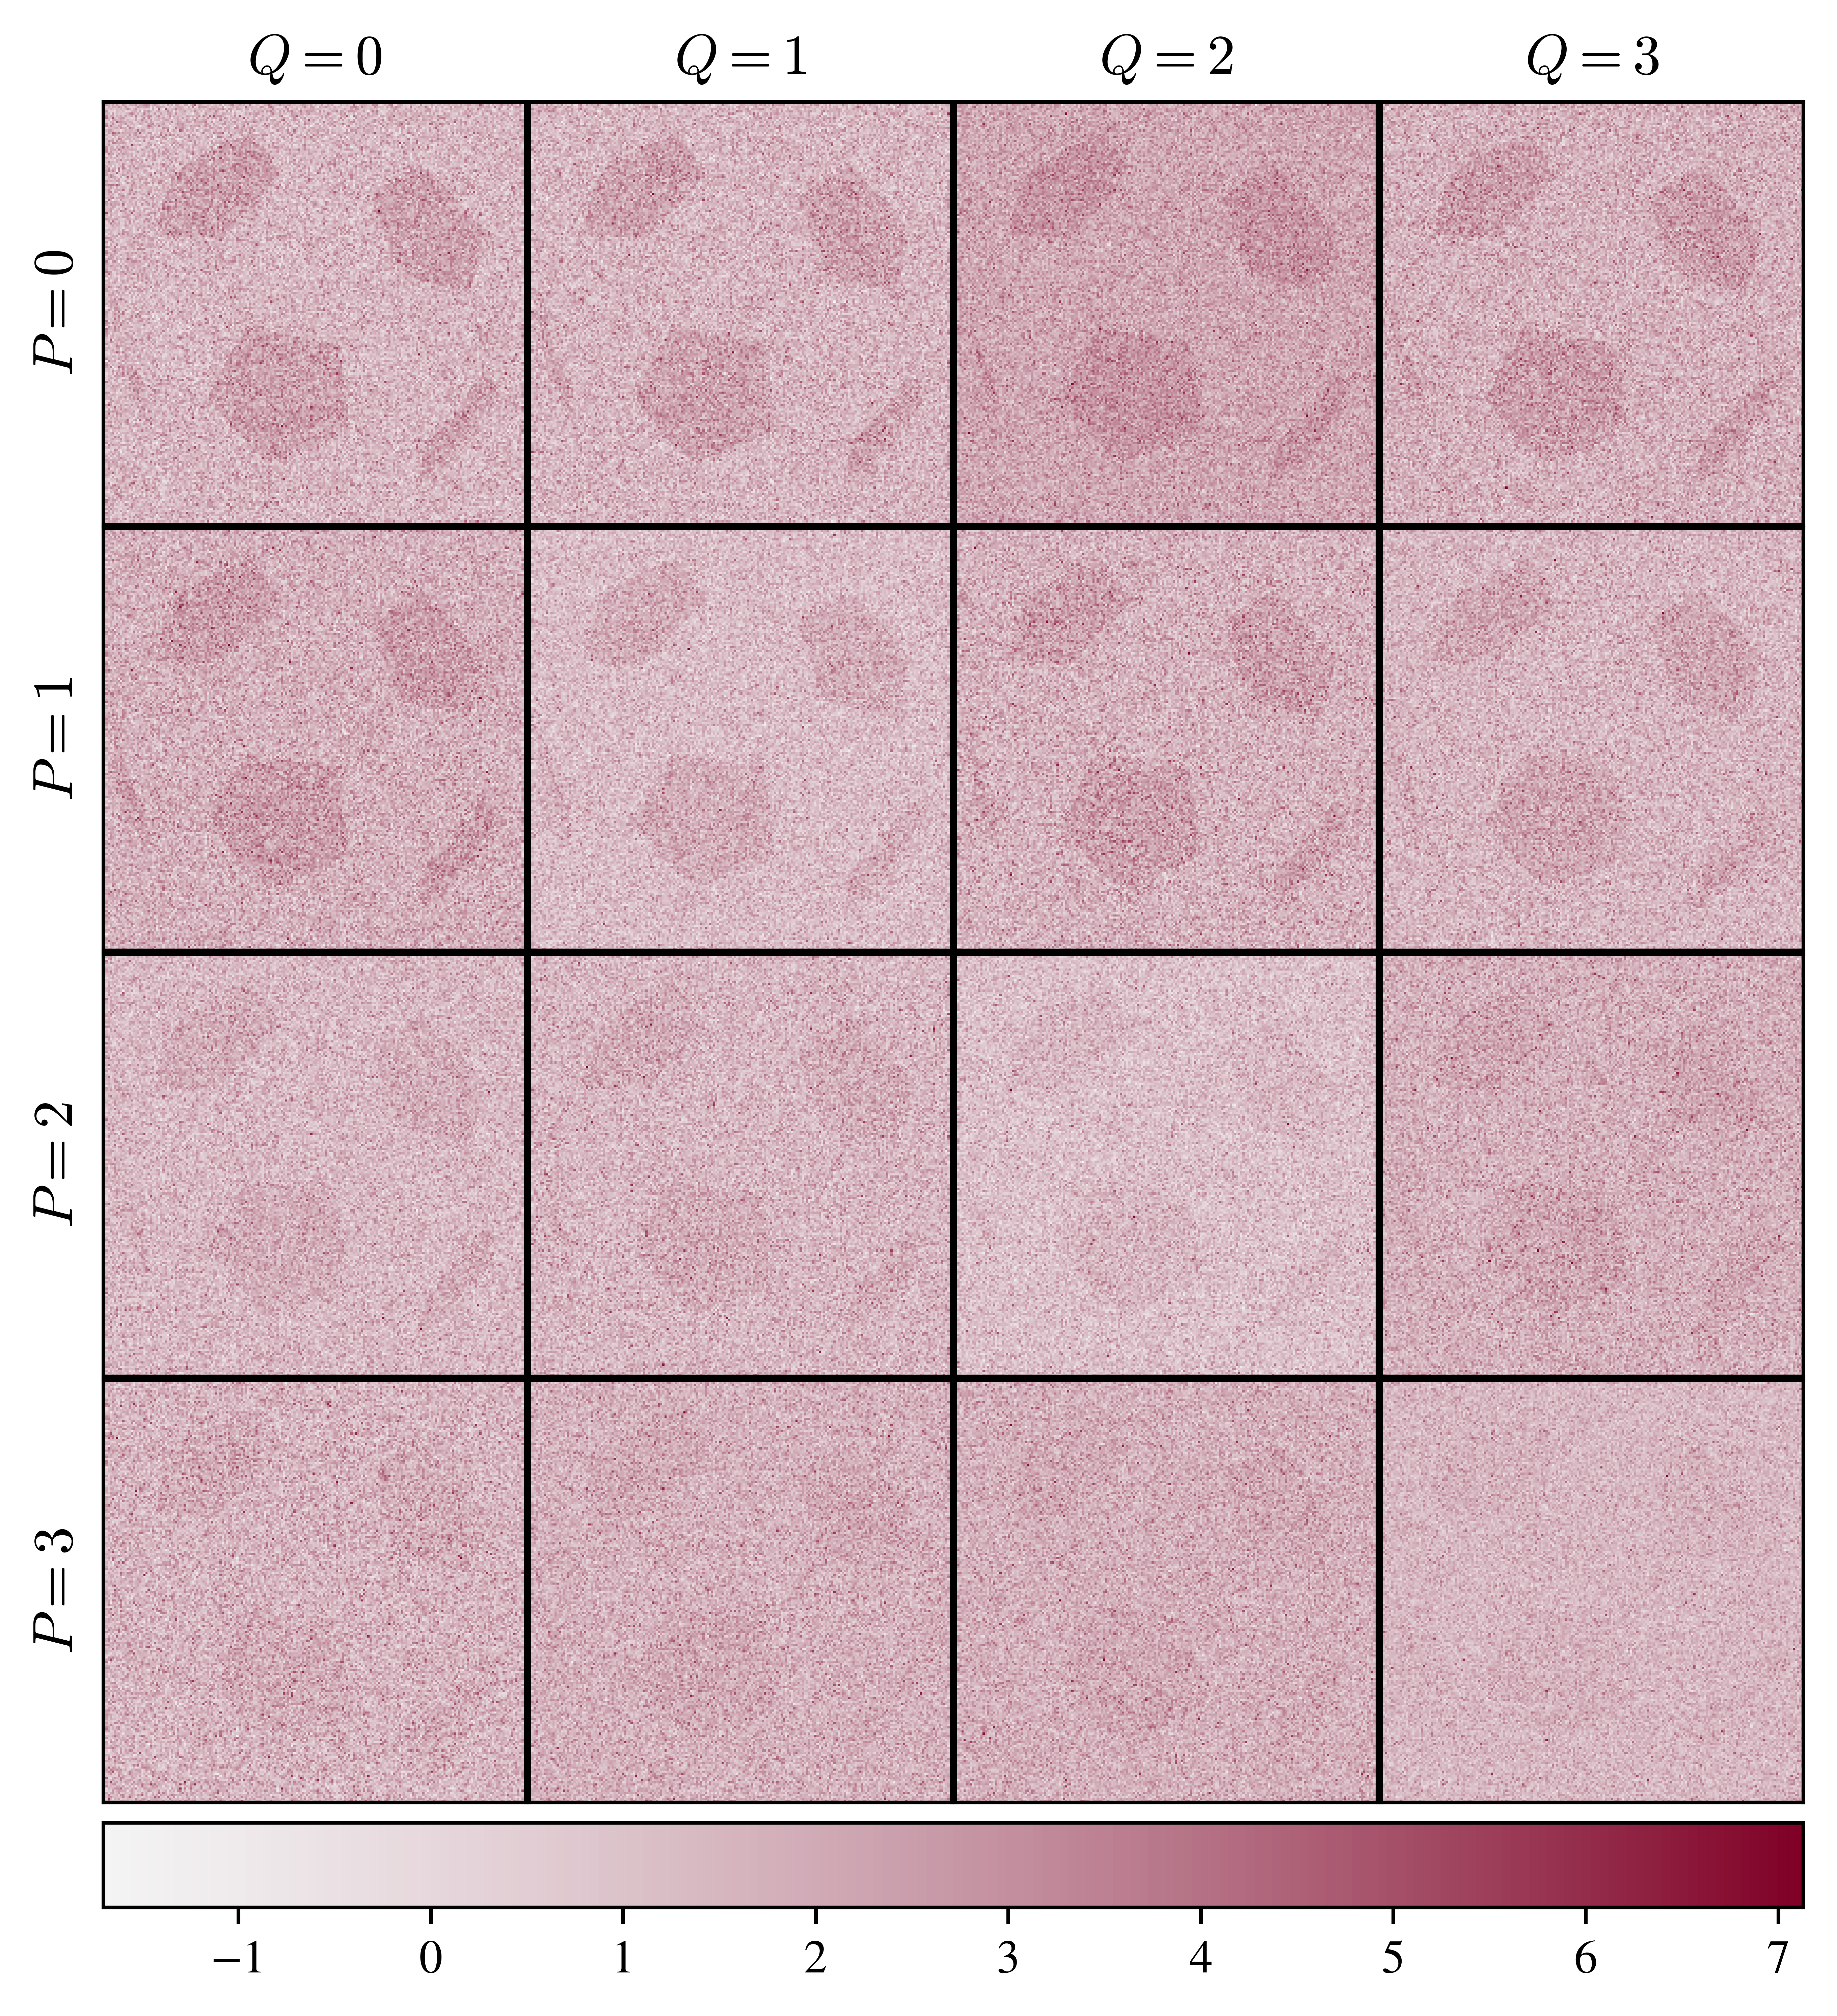
\includegraphics{images/snr2D_Spatial.png}
\caption{Spatial Distribution of the \gls{snr} Values in \gls{2d} Map}
\label{fig:snr2DSpatial}
\end{figure}

\begin{figure}[htbp!]
\centering
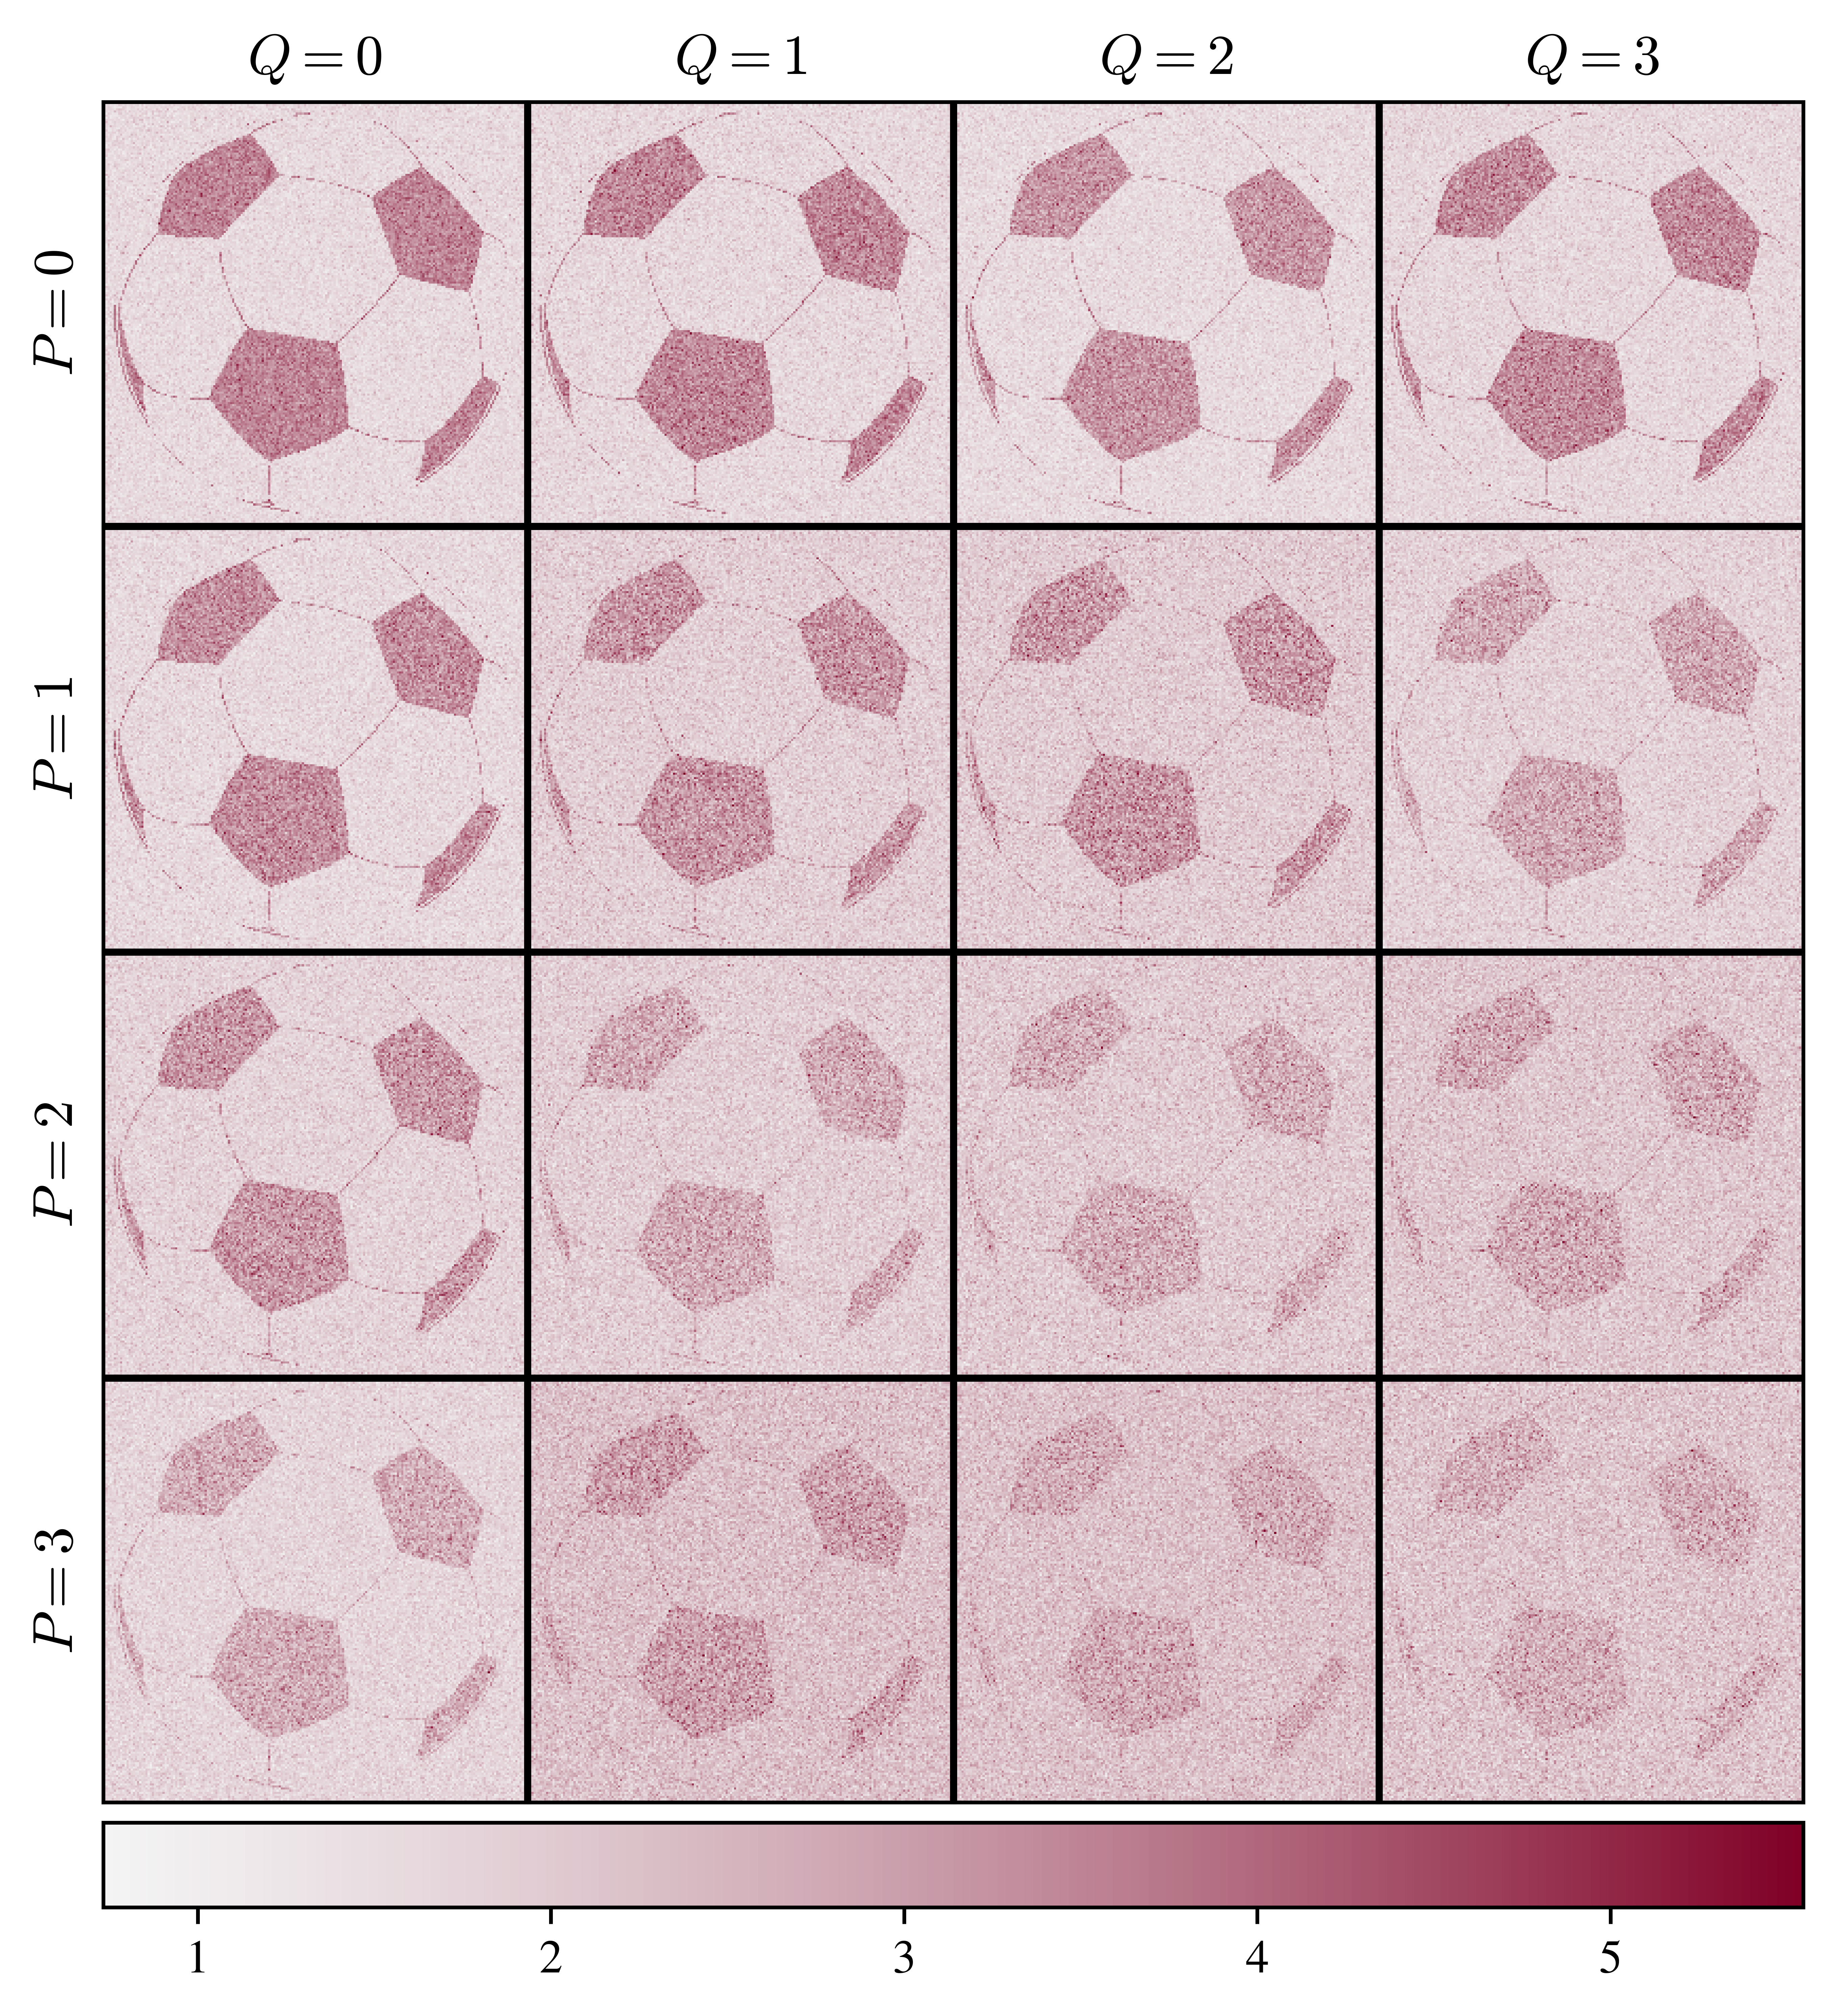
\includegraphics{images/cnr2D_Spatial.png}
\caption{Spatial Distribution of the \gls{cnr} Values in \gls{2d} Map}
\label{fig:cnr2DSpatial}
\end{figure}

\newpage

\section{Example of the Procedure}

In the following figures, examples of the results of probability and activation maps during 
the \gls{bfast} algorithm are shown for $p=0$ and $q=0$. The \gls{2d} case is seen in 
Figure \ref{fig:bfastEx2D} and the $z=20$ plane of the \gls{3d} case is seen in 
Figure \ref{fig:bfastEx3D}.

\begin{figure}[htbp!]
\centering
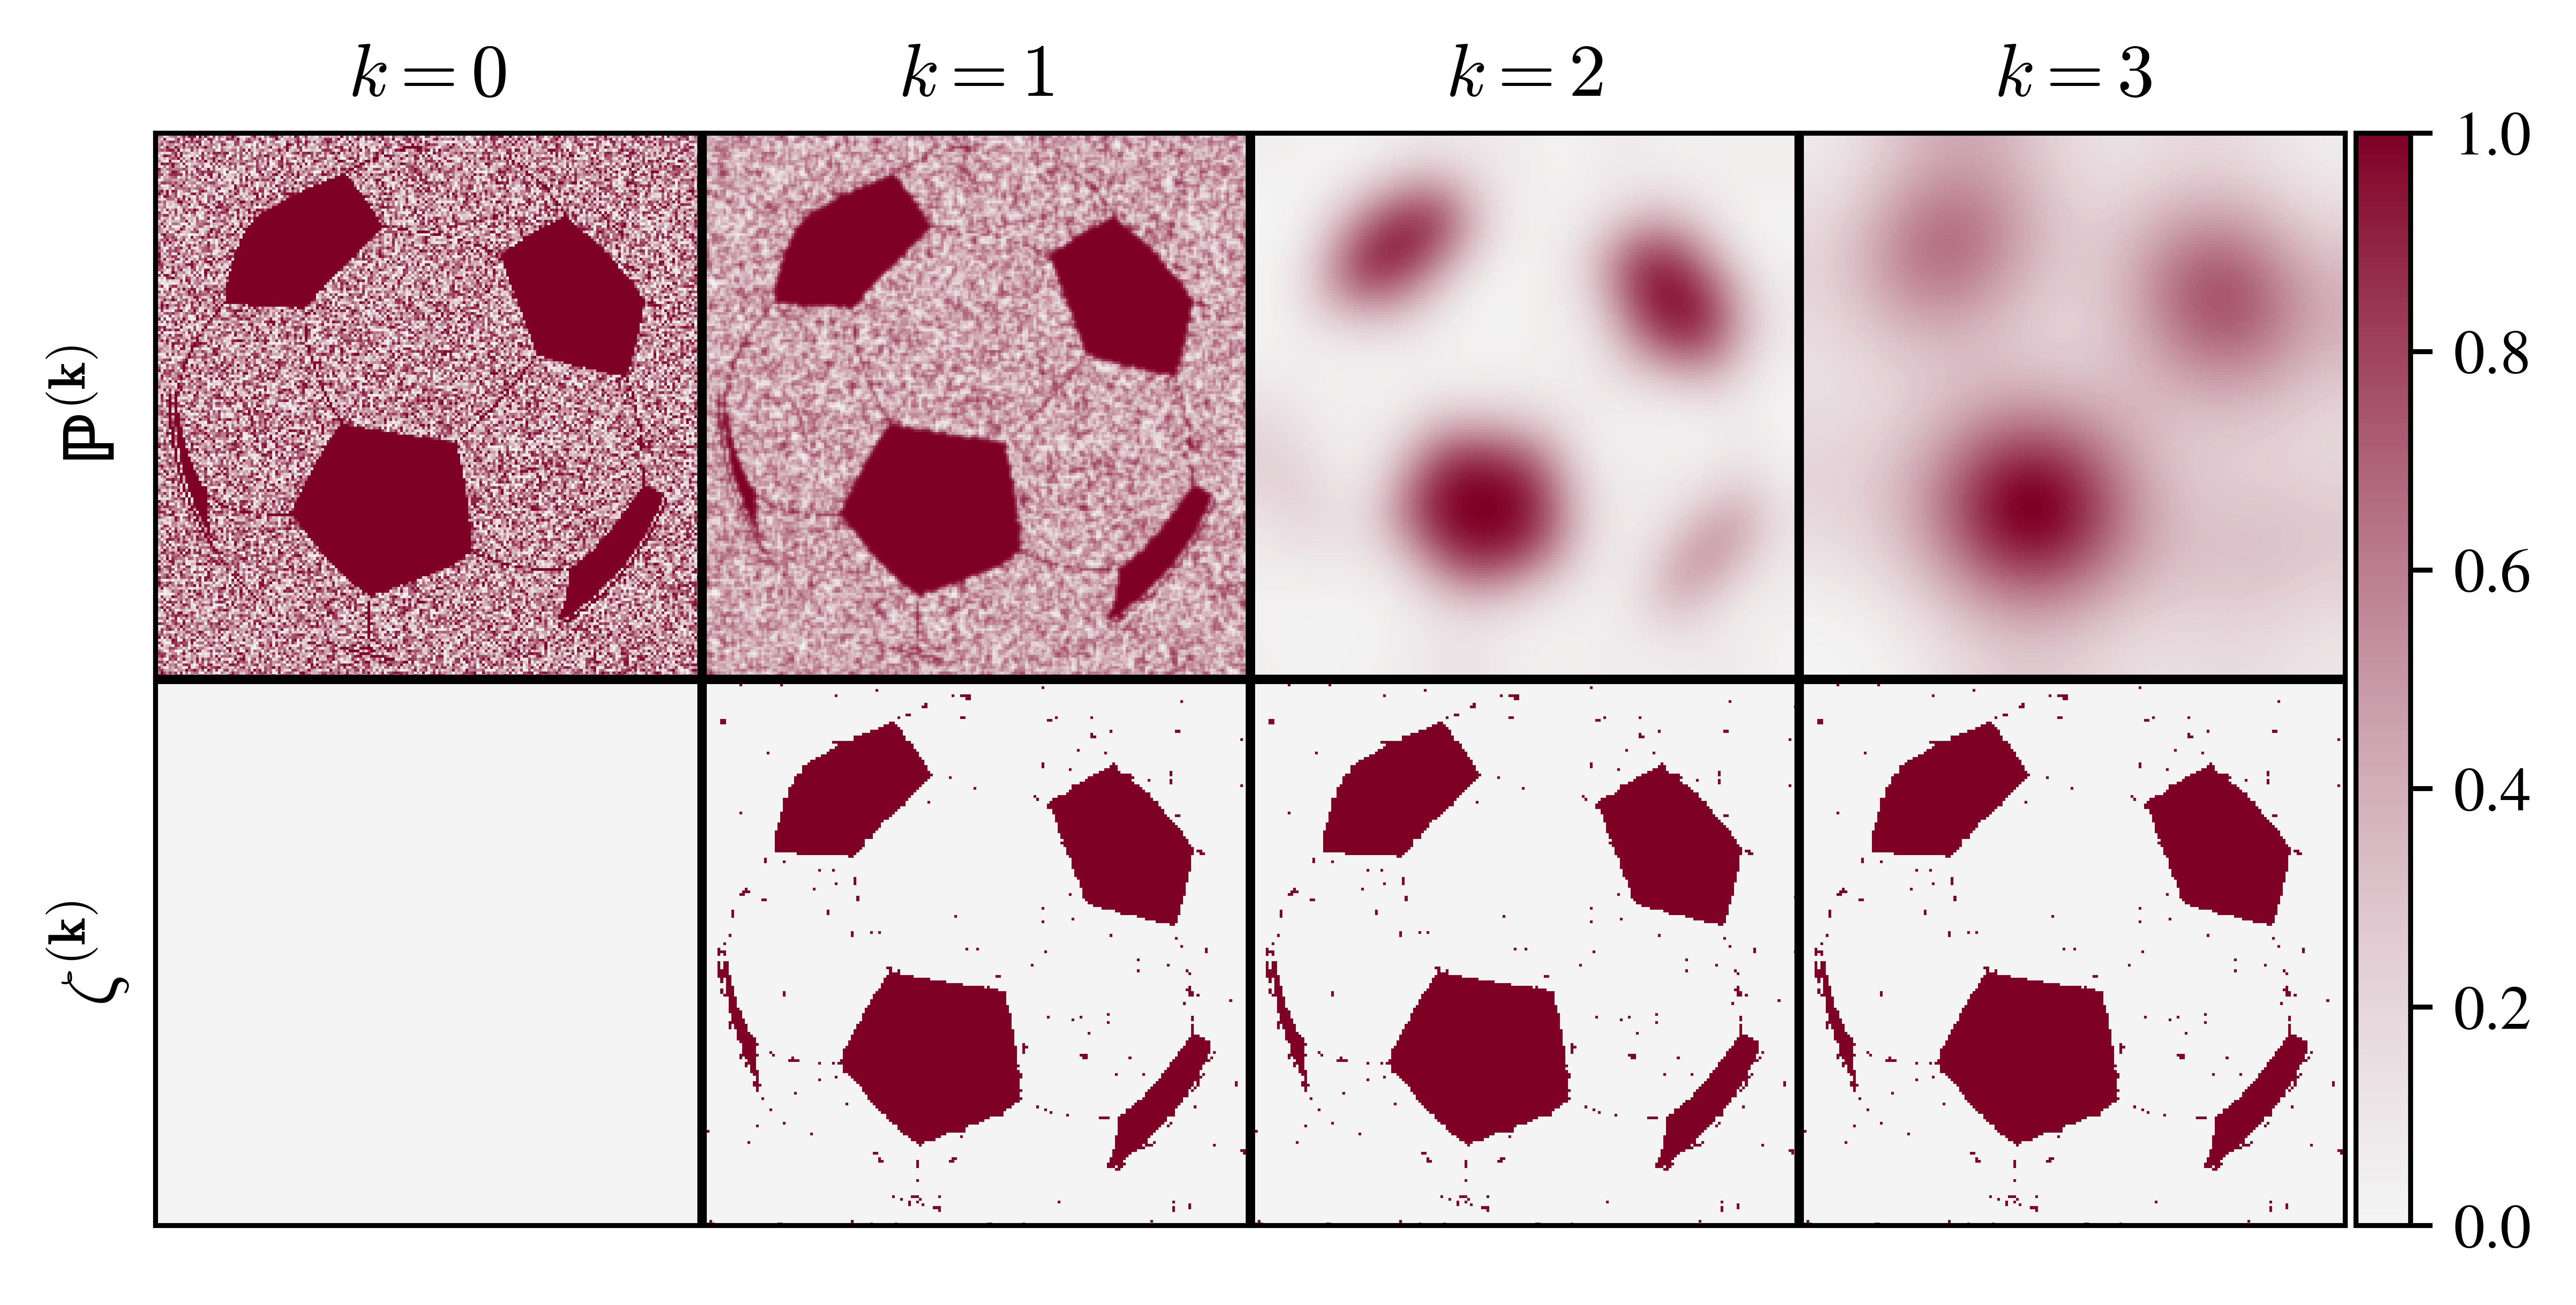
\includegraphics{images/bfastEx2D.png}
\caption{Example of Probability and Activation Maps During \gls{bfast} Algorithm for $p=0$ and $q=0$ in a \gls{2d} Map}
\label{fig:bfastEx2D}
\end{figure}

\begin{figure}[htbp!]
\centering
\includegraphics[width=0.8\textwidth]{images/plot3dSimActPr2.png}
\caption{Example of Probability and Activation Maps During \gls{bfast} Algorithm for $p=0$ and $q=0$ in the \gls{3d} Map}
\label{fig:bfastEx3D}
\end{figure}

\newpage

\section{Performance Metrics}

The performance of the \gls{bfast} algorithm was evaluated by comparing the final activated map with the true activation map using:

\begin{itemize}
\item \gls{ji}: Similarity between the two maps.
\item \gls{fpr}: Ratio of the voxels marked as activated that are not really active and the 
total number of inactive voxels.
\item \gls{poa}: Percentage of active voxels in final activation map. Recall from Table \ref{tab:aMaps} 
that expected values are $19.9375 \%$ and $3.9525 \%$ for the \gls{2d} and \gls{3d} maps, respectively.
\end{itemize}

See Tables \ref{tab:perfSum2D} and \ref{tab:perfSum3D} for the summary of these performance 
metrics in the \gls{2d} and \gls{3d} cases, respectively. Additionally, note from 
Figures \ref{fig:ji2D} and \ref{fig:ji3D} the numerical distribution of
\gls{ji} in each configuration of the simulations in the \gls{2d} and \gls{3d}
cases, respectively. As expected, the accuracy of the \gls{bfast} algorithm decreases 
as the order of the $ARMA$ model increases. However, note that the \gls{ji} in the \gls{2d} case
is around 0.9 and in the \gls{3d} case is around 0.7. These high values confirm that the \gls{bfast}
algorithm has a good performance in different noise scenarios.

\begin{table}[htbp!]
\centering
\caption{Performance Metrics Summary in \gls{2d} Case}
\begin{tabular}{ccccccc}
\hline
\textbf{p} & \textbf{q} & \textbf{\gls{snr}} & \textbf{\gls{cnr}} & \gls{ji} & \gls{fpr} & \gls{poa} \\ \hline
\multirow{4}{*}{0} & 0 & 4.0841 & 3.0344 & 0.9256 & 0.0078 & 19.663 \\
 & 1 & 3.6815 & 2.9342 & 0.8925 & 0.0180 & 20.515 \\
 & 2 & 3.5788 & 2.9035 & 0.8754 & 0.0227 & 20.858 \\
 & 3 & 3.5688 & 2.8960 & 0.8695 & 0.0244 & 20.995 \\ \hline
\multirow{4}{*}{1} & 0 & 3.5988 & 2.9042 & 0.8794 & 0.0222 & 20.870 \\
 & 1 & 2.7538 & 2.6993 & 0.8509 & 0.0299 & 21.398 \\
 & 2 & 2.5159 & 2.6191 & 0.8488 & 0.0308 & 21.475 \\
 & 3 & 2.4691 & 2.6007 & 0.8533 & 0.0292 & 21.350 \\ \hline
\multirow{4}{*}{2} & 0 & 2.9564 & 2.7050 & 0.8685 & 0.0240 & 20.908 \\
 & 1 & 2.1686 & 2.4761 & 0.8648 & 0.0267 & 21.228 \\
 & 2 & 1.8753 & 2.3861 & 0.8578 & 0.0284 & 21.333 \\
 & 3 & 1.8050 & 2.3646 & 0.8581 & 0.0283 & 21.313 \\ \hline
\multirow{4}{*}{3} & 0 & 2.5794 & 2.5607 & 0.8932 & 0.0174 & 20.445 \\
 & 1 & 1.8416 & 2.3420 & 0.8882 & 0.0185 & 20.513 \\
 & 2 & 1.5895 & 2.2576 & 0.8837 & 0.0200 & 20.638 \\
 & 3 & 1.5260 & 2.2323 & 0.8793 & 0.0213 & 20.740 \\ \hline
\end{tabular}
\label{tab:perfSum2D}
\end{table}

\begin{table}[htbp!]
\centering
\caption{Performance Metrics Summary in \gls{3d} Case}
\begin{tabular}{ccccccc}
\hline
\textbf{p} & \textbf{q} & \textbf{\gls{snr}} & \textbf{\gls{cnr}} & \gls{ji} & \gls{fpr} & \gls{poa} \\ \hline
\multirow{4}{*}{0} & 0 & 4.0430 & 2.6156 & 0.7677 & 0.0046 & 3.8075 \\
 & 1 & 3.6401 & 2.5873 & 0.7249 & 0.0068 & 3.9950 \\
 & 2 & 3.5348 & 2.5699 & 0.6796 & 0.0086 & 4.0675 \\
 & 3 & 3.5233 & 2.5660 & 0.6767 & 0.0082 & 3.9950 \\ \hline
\multirow{4}{*}{1} & 0 & 3.5553 & 2.5687 & 0.6741 & 0.0092 & 4.1500 \\
 & 1 & 2.7134 & 2.4836 & 0.6468 & 0.0108 & 4.2650 \\
 & 2 & 2.4711 & 2.4406 & 0.6410 & 0.0116 & 4.3550 \\
 & 3 & 2.4303 & 2.4320 & 0.6757 & 0.0099 & 4.2625 \\ \hline
\multirow{4}{*}{2} & 0 & 2.9143 & 2.4583 & 0.6979 & 0.0083 & 4.1125 \\
 & 1 & 2.1205 & 2.3332 & 0.6566 & 0.0108 & 4.3100 \\
 & 2 & 1.8440 & 2.2791 & 0.6909 & 0.0079 & 4.0075 \\
 & 3 & 1.7735 & 2.2584 & 0.6859 & 0.0081 & 4.0300 \\ \hline
\multirow{4}{*}{3} & 0 & 2.5407 & 2.3554 & 0.7297 & 0.0065 & 3.9650 \\
 & 1 & 1.8073 & 2.2290 & 0.7194 & 0.0067 & 3.9525 \\
 & 2 & 1.5582 & 2.1729 & 0.7167 & 0.0074 & 4.0600 \\
 & 3 & 1.5004 & 2.1515 & 0.7092 & 0.0066 & 3.8925 \\ \hline
\end{tabular}
\label{tab:perfSum3D}
\end{table}

\begin{figure}[htbp!]
\centering
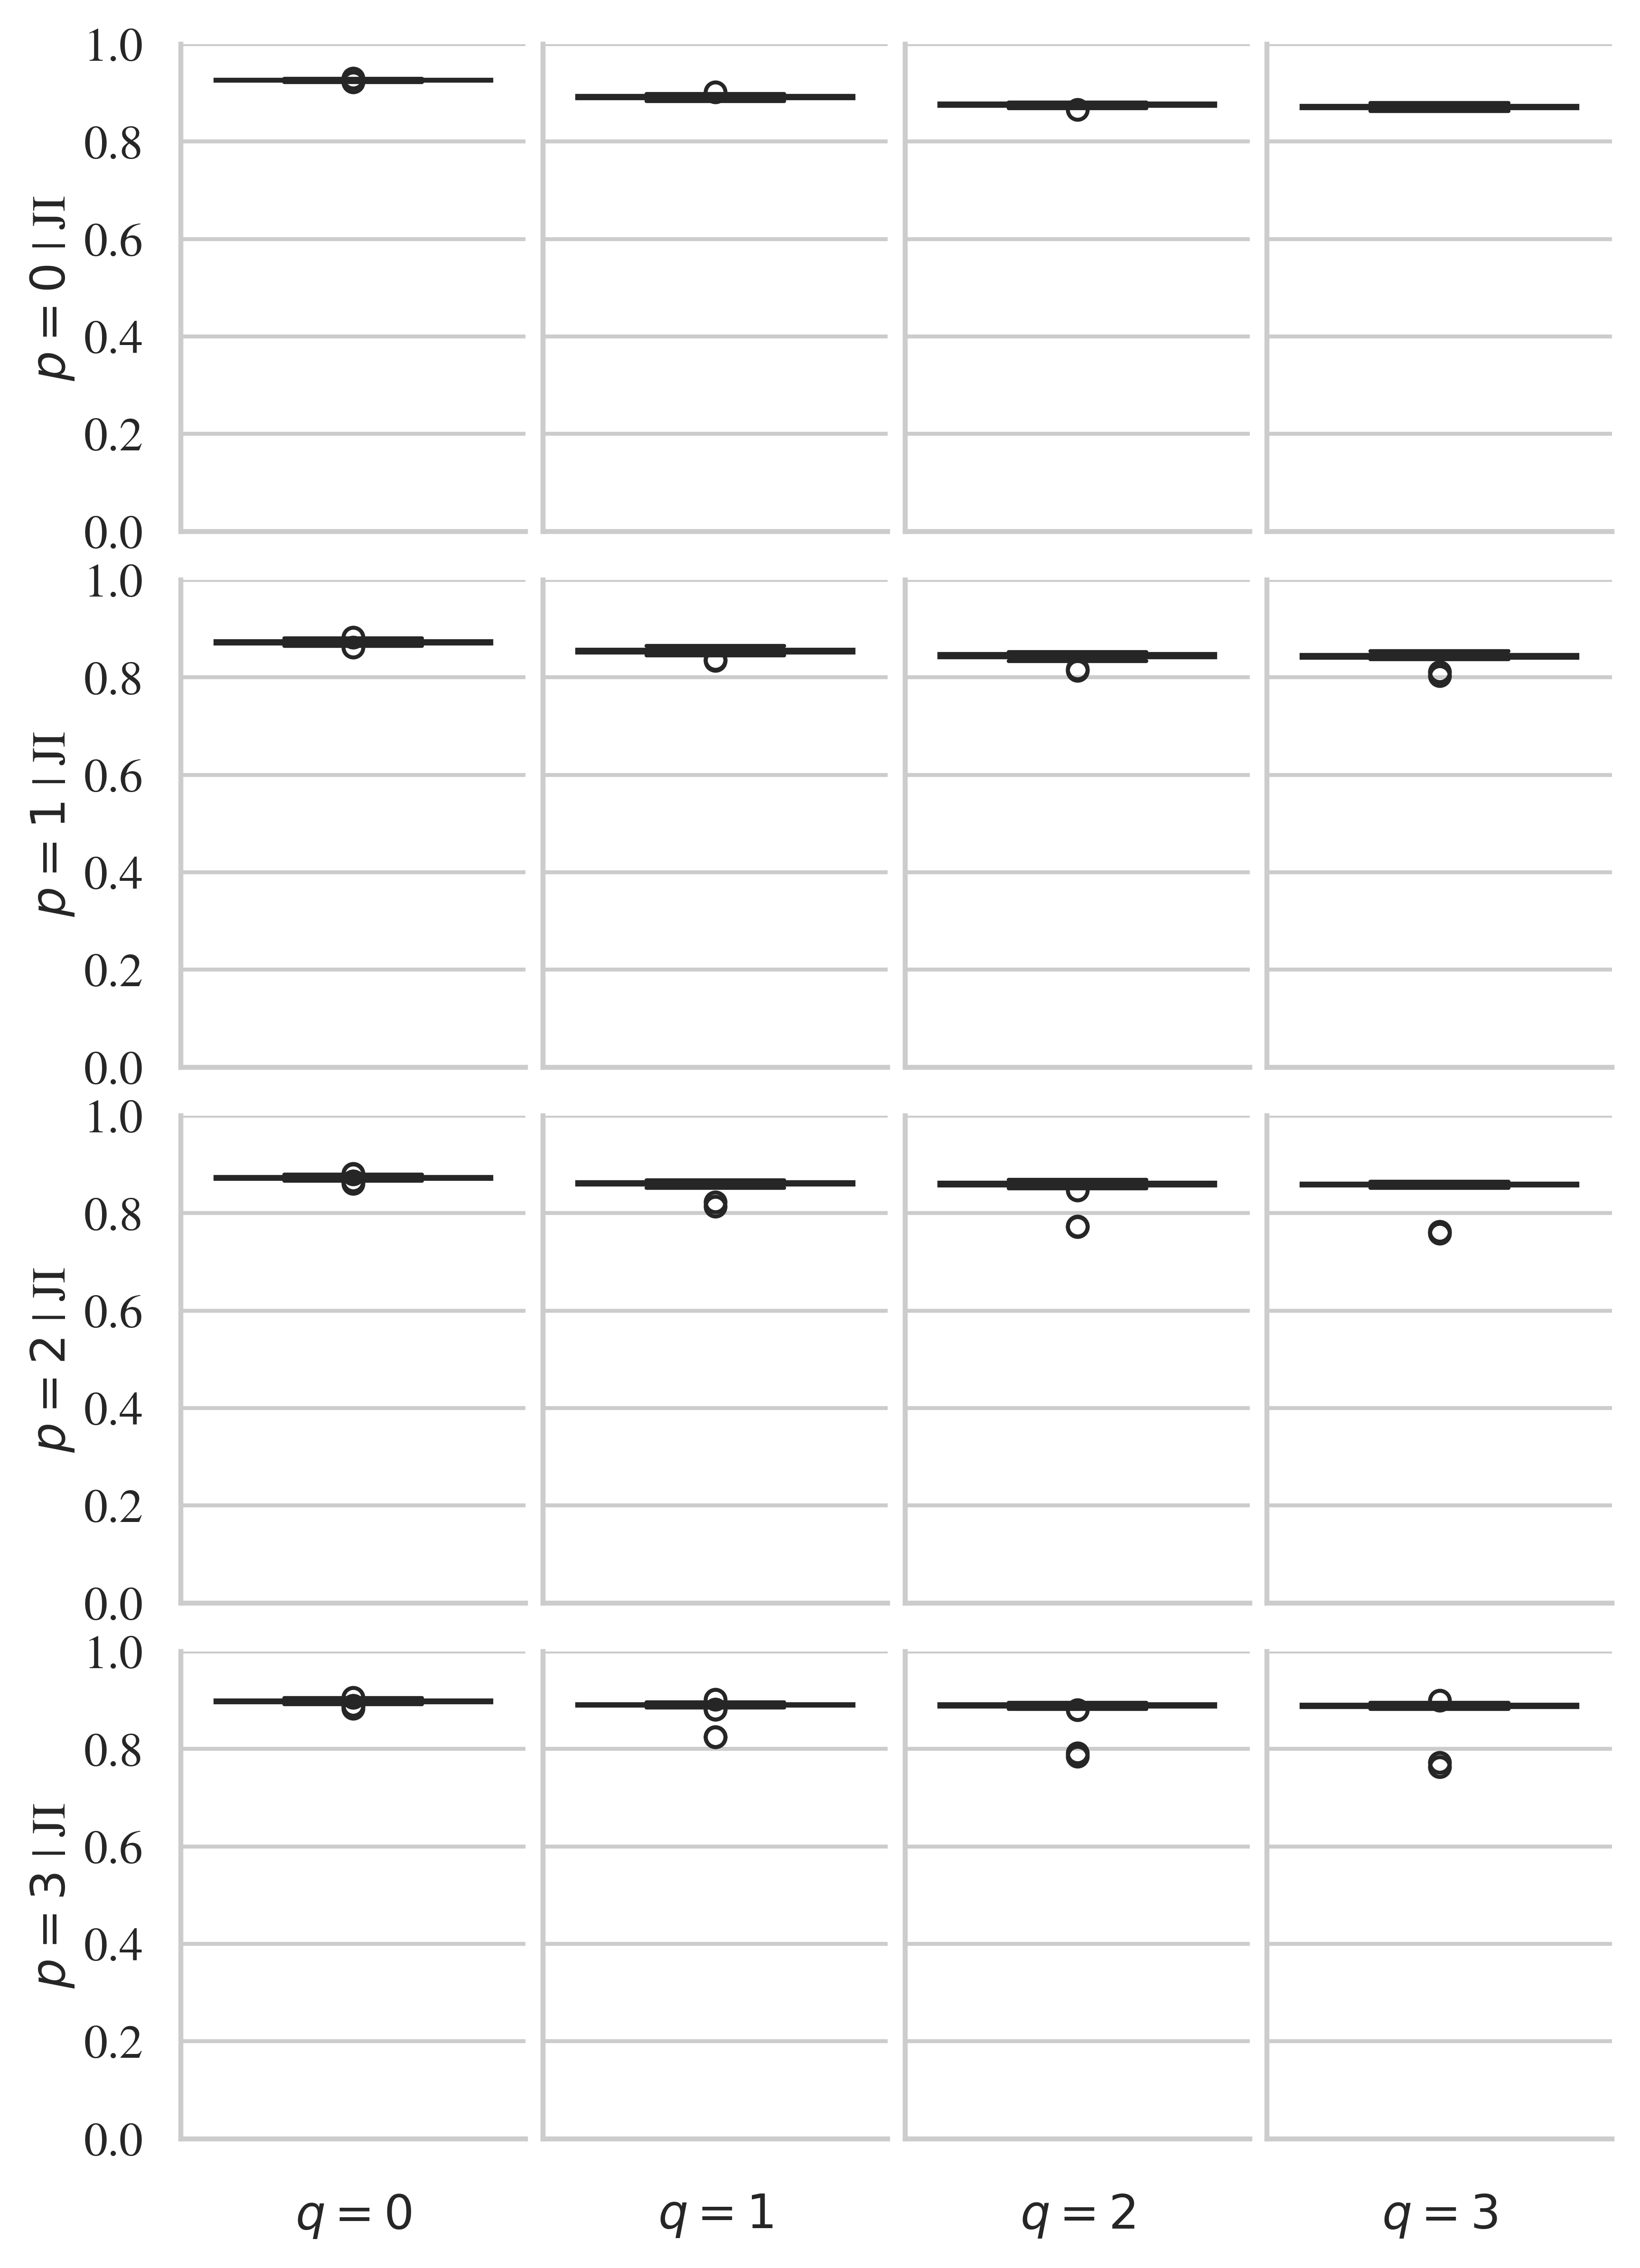
\includegraphics{images/ji2D.png}
\caption{Numerical Distribution of the \gls{ji} Values in \gls{2d} Map}
\label{fig:ji2D}
\end{figure}

\begin{figure}[htbp!]
\centering
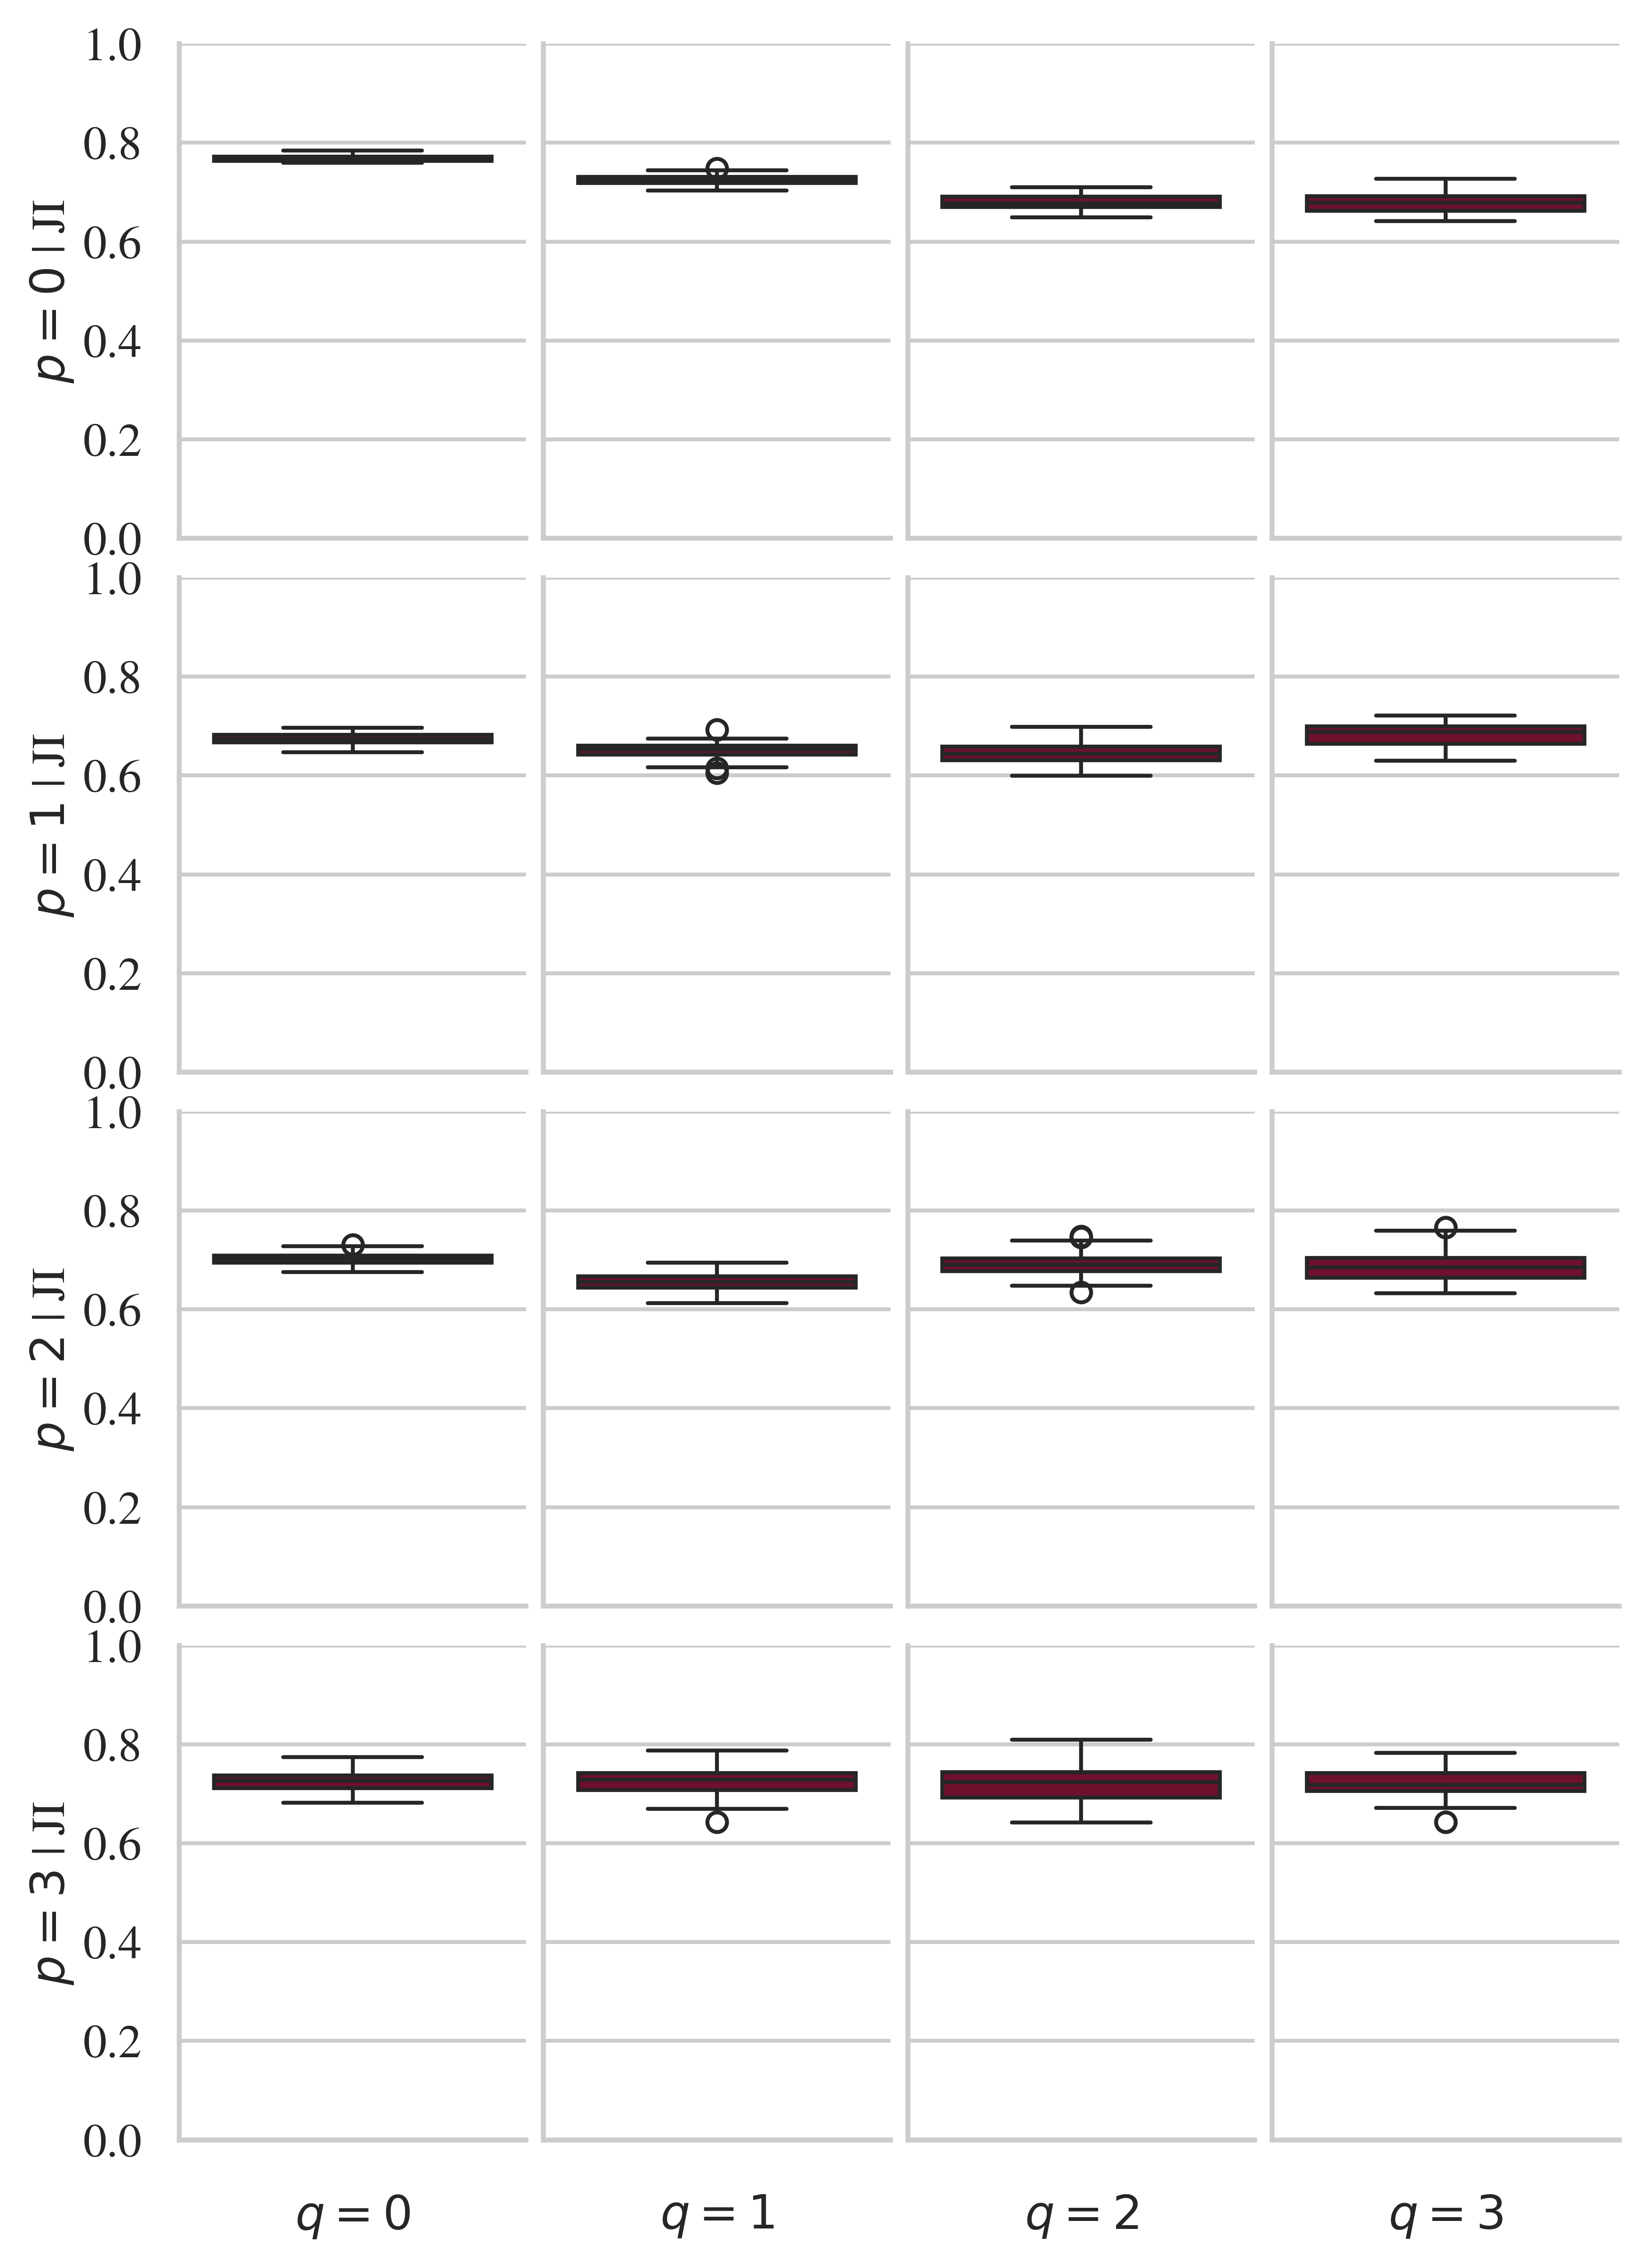
\includegraphics{images/ji3D.png}
\caption{Numerical Distribution of the \gls{ji} Values in \gls{3d} Map}
\label{fig:ji3D}
\end{figure}